
 % \IEEEoverridecommandlockouts
 % % The line before this one is solely needed to find the financing in the first footnote.  If you don't require it, please comment it out.
 % \usepackage{float}
 % \usepackage{cite}
 % \usepackage{amsmath, amssymb, amsfonts}
 % \usepackage{algorithmic}
 % \usepackage{graphicx}
 % \usepackage{textcomp}
 % \usepackage{xcolor}
 % \def\BibTeX{{\rm B\kern-.05em{\sc i\kern-.025em b}\kern-.08em
 % T\kern-.1667em\lower.7ex\hbox{E}\kern-.125emX
 % \begin{document}

 % A Stacked Ensemble Learning Approach for Hyper-Local PM2.5 Prediction Utilizing Satellite AOD and Meteorological Data

 % \author{\IEEEauthorblockN{1\textsuperscript{st} Md.  Masum Billah
 % \IEEEauthorblockA{\textit{Department of Computer Science and Engineering} \\
 % Bangladesh University of Business and Technology (BUBT)
 % Bangladesh, Dhaka
 % md.masum.cse.bd@gmail.com}
 % And
 % \IEEEauthorblockN{2nd Md.  Syfulla
 % \IEEEauthorblockA{\textit{Department of Computer Science and Engineering} \\
 % Bangladesh University of Business and Technology (BUBT)
 % Dhaka, Bangladesh
 % syfullasanto122@gmail.com
 % and
 % 3rd Chowdhury Kashfee Kamal Fagun
 % \IEEEauthorblockA{\textit{Department of Computer Science and Engineering} \\
 % Bangladesh University of Business and Technology (BUBT)
 % Dhaka, Bangladesh
 % kashfee368@gmail.com}
 % and
 % 4th Tanveer Rabbani
 % \IEEEauthorblockA{\textit{Computer Science and Engineering Department} \\
 % Bangladesh University of Business and Technology (BUBT)
 % Bangladesh's capital, Dhaka
 % tanveerrabbani2002@gmail.com
 % and
 % \IEEEauthorblockN{5\textsuperscript{th} Md.  Jahidul Islam
 % \IEEEauthorblockA{\textit{Department of Computer Science and Engineering} \\
 % Bangladesh University of Business and Technology (BUBT)
 % Bangladesh, Dhaka
 % jahidislam1204.bd@gmail.com

 % }

 % \maketitle


 % In this abstract
 % To control air quality well, it is very important to detect fine particulate matter (PM$_{2.5}$) correctly at a very small scale.  Nonetheless, this persists as a challenge because to the restricted spatial coverage of terrestrial monitoring stations.  This study presents an ensemble-based machine learning architecture that integrates many data sources, including ground-level PM$_{2.5}$ measurements, satellite-derived Aerosol Optical Depth (AOD), meteorological variables, and geographic information.  We use Random Forest and XGBoost regressors as foundation learners that work together.  A meta-model based on linear regression combines their predictions to come up with final PM$_{2.5}$ estimates.

 % We employ standard regression measures to test the proposed framework on a set of data that was not used during training.  The ensemble model gets a \textbf{$R^2$ value of roughly 0.56}, which is better than the individual base models.  This shows that using complementary learners together works well for predicting PM$_{2.5}$ in areas with little data.  Feature importance analysis shows that the amount of AOD from satellites and the position in space are two of the most important things that determine the amount of PM₂.₅.

 % To show how useful it is in the real world, the trained ensemble model is used as a real-time Flask-based application programming interface (API) that uses live weather data to make real-time predictions for PM2.5 and Air Quality Index (AQI) categories.  The findings demonstrate that lightweight ensemble learning combined with heterogeneous data fusion offers an efficient and comprehensible method for hyperlocal air quality estimation.

 % \end{abstract


 % \section{INTRODUCTION

 % The deterioration of air quality is a significant environmental and public health issue of our era.  This is especially true in places that are turning into cities and industry very quickly.  Fine particulate matter (PM$_{2.5}$) is one of the worst air pollutants because it can get deep into the lungs and bloodstream, causing heart and lung problems, early death, and a shorter life span.  It is very important to keep an eye on and precisely estimate the levels of PM$_{2.5}$ so that the air stays clean, rules are made, and health warnings are sent out on time.

 % Most old-fashioned air quality monitoring systems use sensor networks on the ground to get precise and consistent readings of contaminants.  But these monitoring stations don't cover very much territory because they are expensive to set up and keep running, especially in developing countries and areas near cities.  This poor coverage makes it hard to see small changes in air pollution and hard to build continuous, high-resolution PM$_{2.5}$ maps that are needed for hyper-local air quality monitoring and making smart choices.

 % Satellite remote sensing is another option because it can cover enormous areas of land all the time and in great detail.  Satellite-derived Aerosol Optical Depth (AOD) is often used as a stand-in for atmospheric aerosol loading. It has been proven to have a strong link to PM$_{2.5}$ at ground level when the weather is right.  However, AOD alone cannot properly describe the amounts of particulate matter near the surface because it is affected by things like relative humidity, cloud cover, and the vertical dispersion of aerosols.  So, to get an accurate estimate of PM$_{2.5}$, satellite measurements need to be combined with weather and geography data.

 % Recent progress in machine learning has made it possible for data-driven methods to find complicated and nonlinear links between several environmental factors.  Ensemble learning approaches, which use more than one model to make predictions more accurate and reliable, have shown a lot of promise in tasks that involve predicting air quality.  Tree-based models like Random Forest and XGBoost are especially good for this problem since they can handle different types of data, find nonlinear relationships, and work well even when there isn't much data.  When put together in an ensemble framework, these models can use their strengths to balance out the weaknesses of each model.

 % This research puts forward an ensemble-based machine learning framework for hyper-local PM$_{2.5}$ prediction by combining many types of data, such as ground-level PM$_{2.5}$ observations, satellite-derived Aerosol Optical Depth (AOD), weather data, and geographic information.  The framework uses Random Forest and XGBoost regressors as base learners. A meta-model based on linear regression combines their outputs to give final PM$_{2.5}$ estimations.  The proposed architecture is easy to understand, doesn't use a lot of resources, and is light, making it a good choice for real-time use in places with limited resources and data.

 % We use a held-out test dataset and standard regression performance indicators to test the proposed methodology.  The findings indicate that the ensemble method produces more precise predictions compared to standalone base models.  The system's practical usefulness is shown even further by the fact that it is used as a real-time Flask-based application programming interface (API) that uses live weather data to make real-time PM$_{2.5}$ predictions and show the associated Air Quality Index (AQI) categories.  The goal of this effort is to come up with a scalable and useful way to estimate hyper-local air quality by integrating lightweight ensemble learning, heterogeneous data fusion, and real-time operational deployment.

 % What This Work Adds

 % The key contributions of this research can be summed up as follows:

 % \begin{itemize}
 % A method for combining ground-based PM$_{2.5}$ measurements, satellite-derived AOD, weather data, and geographic information to make hyper-local air quality assessments.
 % An ensemble-based PM$_{2.5}$ prediction system that uses a linear regression meta-model to integrate Random Forest and XGBoost regressors. This makes the predictions better than those made by each base learner on its own.
 % An empirical feature importance study showing that AOD from satellites and where it is located in space are the most important elements that affect PM$_{2.5}$ levels at ground level.
 % A real-time implementation of the trained ensemble model as a Flask-based API that uses live weather data to make real-time predictions about PM2.5 levels and AQI categories, showing how useful it is in the real world.
 % \end{itemize}

 % \end{enumerate}

 % \section{Review of the Literature}
 % Méndez et al. \cite{b1} present a comprehensive survey of machine learning techniques for air quality forecasting from 2011 to 2021.  They looked at 155 studies that compared regression models (ARIMA, SVR, RF) and deep learning approaches (MLP, CNN, LSTM).  The results demonstrated that LSTM-based models surpass conventional methods by more effectively capturing temporal dependence and nonlinearity in pollution trends.  The study, on the other hand, pointed out problems such not having enough data, the high cost of computing, and the fact that models are hard to understand.


 % Zhang et al. \cite{b2} present a comprehensive examination of air quality forecasting utilizing deep learning methodologies.  The research assesses air quality forecasting techniques by contrasting conventional numerical and statistical models with contemporary deep learning methodologies, including CNN, RNN, LSTM, and GCN. It examines the capacity of these models to manage temporal, spatial, and spatiotemporal dependencies in pollutant data to enhance forecasting precision for critical indicators such as PM2.5, PM10, and AQI.  The article showed that deep learning methods are better than traditional models at finding nonlinear and complicated pollution patterns.  It also talked about big problems like not having enough data, not being able to understand models, and how hard it is to do math. 

 % Lee et al. \cite{b3} created a deep neural network that can use different training data to forecast the average PM2:5 levels for the next two days.  They combined ground-based observation data with data from numerical models (CMAQ and WRF) to generate a hybrid dataset (DNN-ALL) for training.  The model was far better at making predictions than the CMAQ model on its own, as seen by the lower RMSE.  It depends on what the NWP/AQ models that need a lot of computer power say.  There is an urgent requirement for autonomous, data-driven systems capable of attaining high accuracy and delivering assurance independently, hence enhancing system scalability and real-time inference speed.

 % Pan et al. \cite{b4} introduced a Graph Attention Recurrent Neural Network (GARNN) model for predicting PM2.5 levels in 308 Chinese cities, utilizing data from 2015 to 2022.  Their model coupled an attention-based graph neural network with a gated recurrent unit (GRU) to successfully capture spatial and temporal correlations among meteorological and pollution data.   The suggested framework was better at making predictions than regular LSTM, GRU, and GC-LSTM models since it had lower RMSE and MAE values.  The model works best with big datasets and a lot of computing power, which makes it hard to use in real time.

 % Zhang et al. \cite{b5} created a Sparse Attention-based Transformer Network (STN) to make PM2.5 predictions better.  The model uses encoder-decoder layers with multi-head sparse attention to quickly find long-term trends in time.  When tested on datasets from Beijing and Taizhou, STN got R² values of 0.937 and 0.924, which means it was more accurate than other models like LSTM, GRU, and Standard Transformers.  Because it needs a lot of data and computing power, it can't be used in real-time or data-scarce situations. This shows how important it is to have lightweight and easy-to-understand models.


 % Qi et al. \cite{b6} put forward a hybrid model for predicting PM2.5 levels over time and space using a graph convolutional neural network and long short-term memory concentrations in the Jing-Jin-Ji region of China.  The models clearly show how air pollution data is related to both space and time.  The model did better than traditional methods, getting excellent accuracy (R² = 0.91 for 1-hour forecasts and R² = 0.72 for 72-hour forecasts) in predicting PM2.5 levels in North China.  This method relies on fixed monitoring infrastructures and does not incorporate satellite, traffic, or emission data, which are essential for thorough air quality assurance and early warning systems.

 % Utku et al. \cite{b7} provide a hybrid deep learning model that integrates Convolutional Neural Networks (CNNs) and Recurrent Neural Networks (RNNs) for estimating "PM$_{2.5}$" concentration.  The model was made to easily capture both spatial and temporal correlations in air quality data while keeping the math simple.  The model was tested on datasets from India, Milan, and Frankfurt and got R² values as high as 0.995, which was better than CNN, LSTM, and CNN-LSTM baselines.  This investigation showed that the model is strong and can be used in a wide range of weather conditions.  This method is mostly based on ground-based and weather data, and it doesn't include satellite or emission sources that are needed for a full air quality check.

 % Bhanja and Das \cite{b8} put forward a hybrid deep learning model for predicting air quality time series by combining Convolutional Neural Networks (CNNs) with Bidirectional Long Short-Term Memory (BDLSTM) networks.  The model employed a 3D tensor construction approach to successfully represent spatial and temporal dependencies.  It had the lowest RMSE and MAPE of all the benchmark models when tested on the Sydney and Delhi datasets.  The method was quite accurate and stable, but it only worked for single-step forecasting and didn't work with satellite or emission data to fully ensure air quality.

 % \section{Methodology

 % \subsection{System Structure and Architecture}
 % This study's proposed air quality prediction system is based on a Stacked Generalization (Ensemble Learning) architecture.  This method takes the predictions of several different models, called "base-models" or "experts," and puts them into a final "meta-model" to make a more reliable and accurate final forecast.

 % There are three basic hierarchical layers in the system structure:
 % 1.
 % 1. The Data Acquisition and Preprocessing Layer is in charge of collecting both ground-truth and satellite/weather data, fixing any missing entries, and getting the feature set ready.
 % Base Model Layer (Ensemble Experts): Two different machine learning models were trained on the main feature set to make early predictions:
 % \begin{itemize}
 % Random Forest Regressor (RF)
 % XGBoost Regressor (XGB)
 % \end{itemize}
 % A Linear Regression model acts as the stacking manager, using the outputs of the two basic models as its input features to make the final, best PM2.5 forecast.
 % \end{enumerate}



 % % --- PUT THIS IN FOR IMAGE 1 (Stacking Architecture) ---
 % \begin{figure}[H] % [H] keeps it exactly here
 % \centering
 % 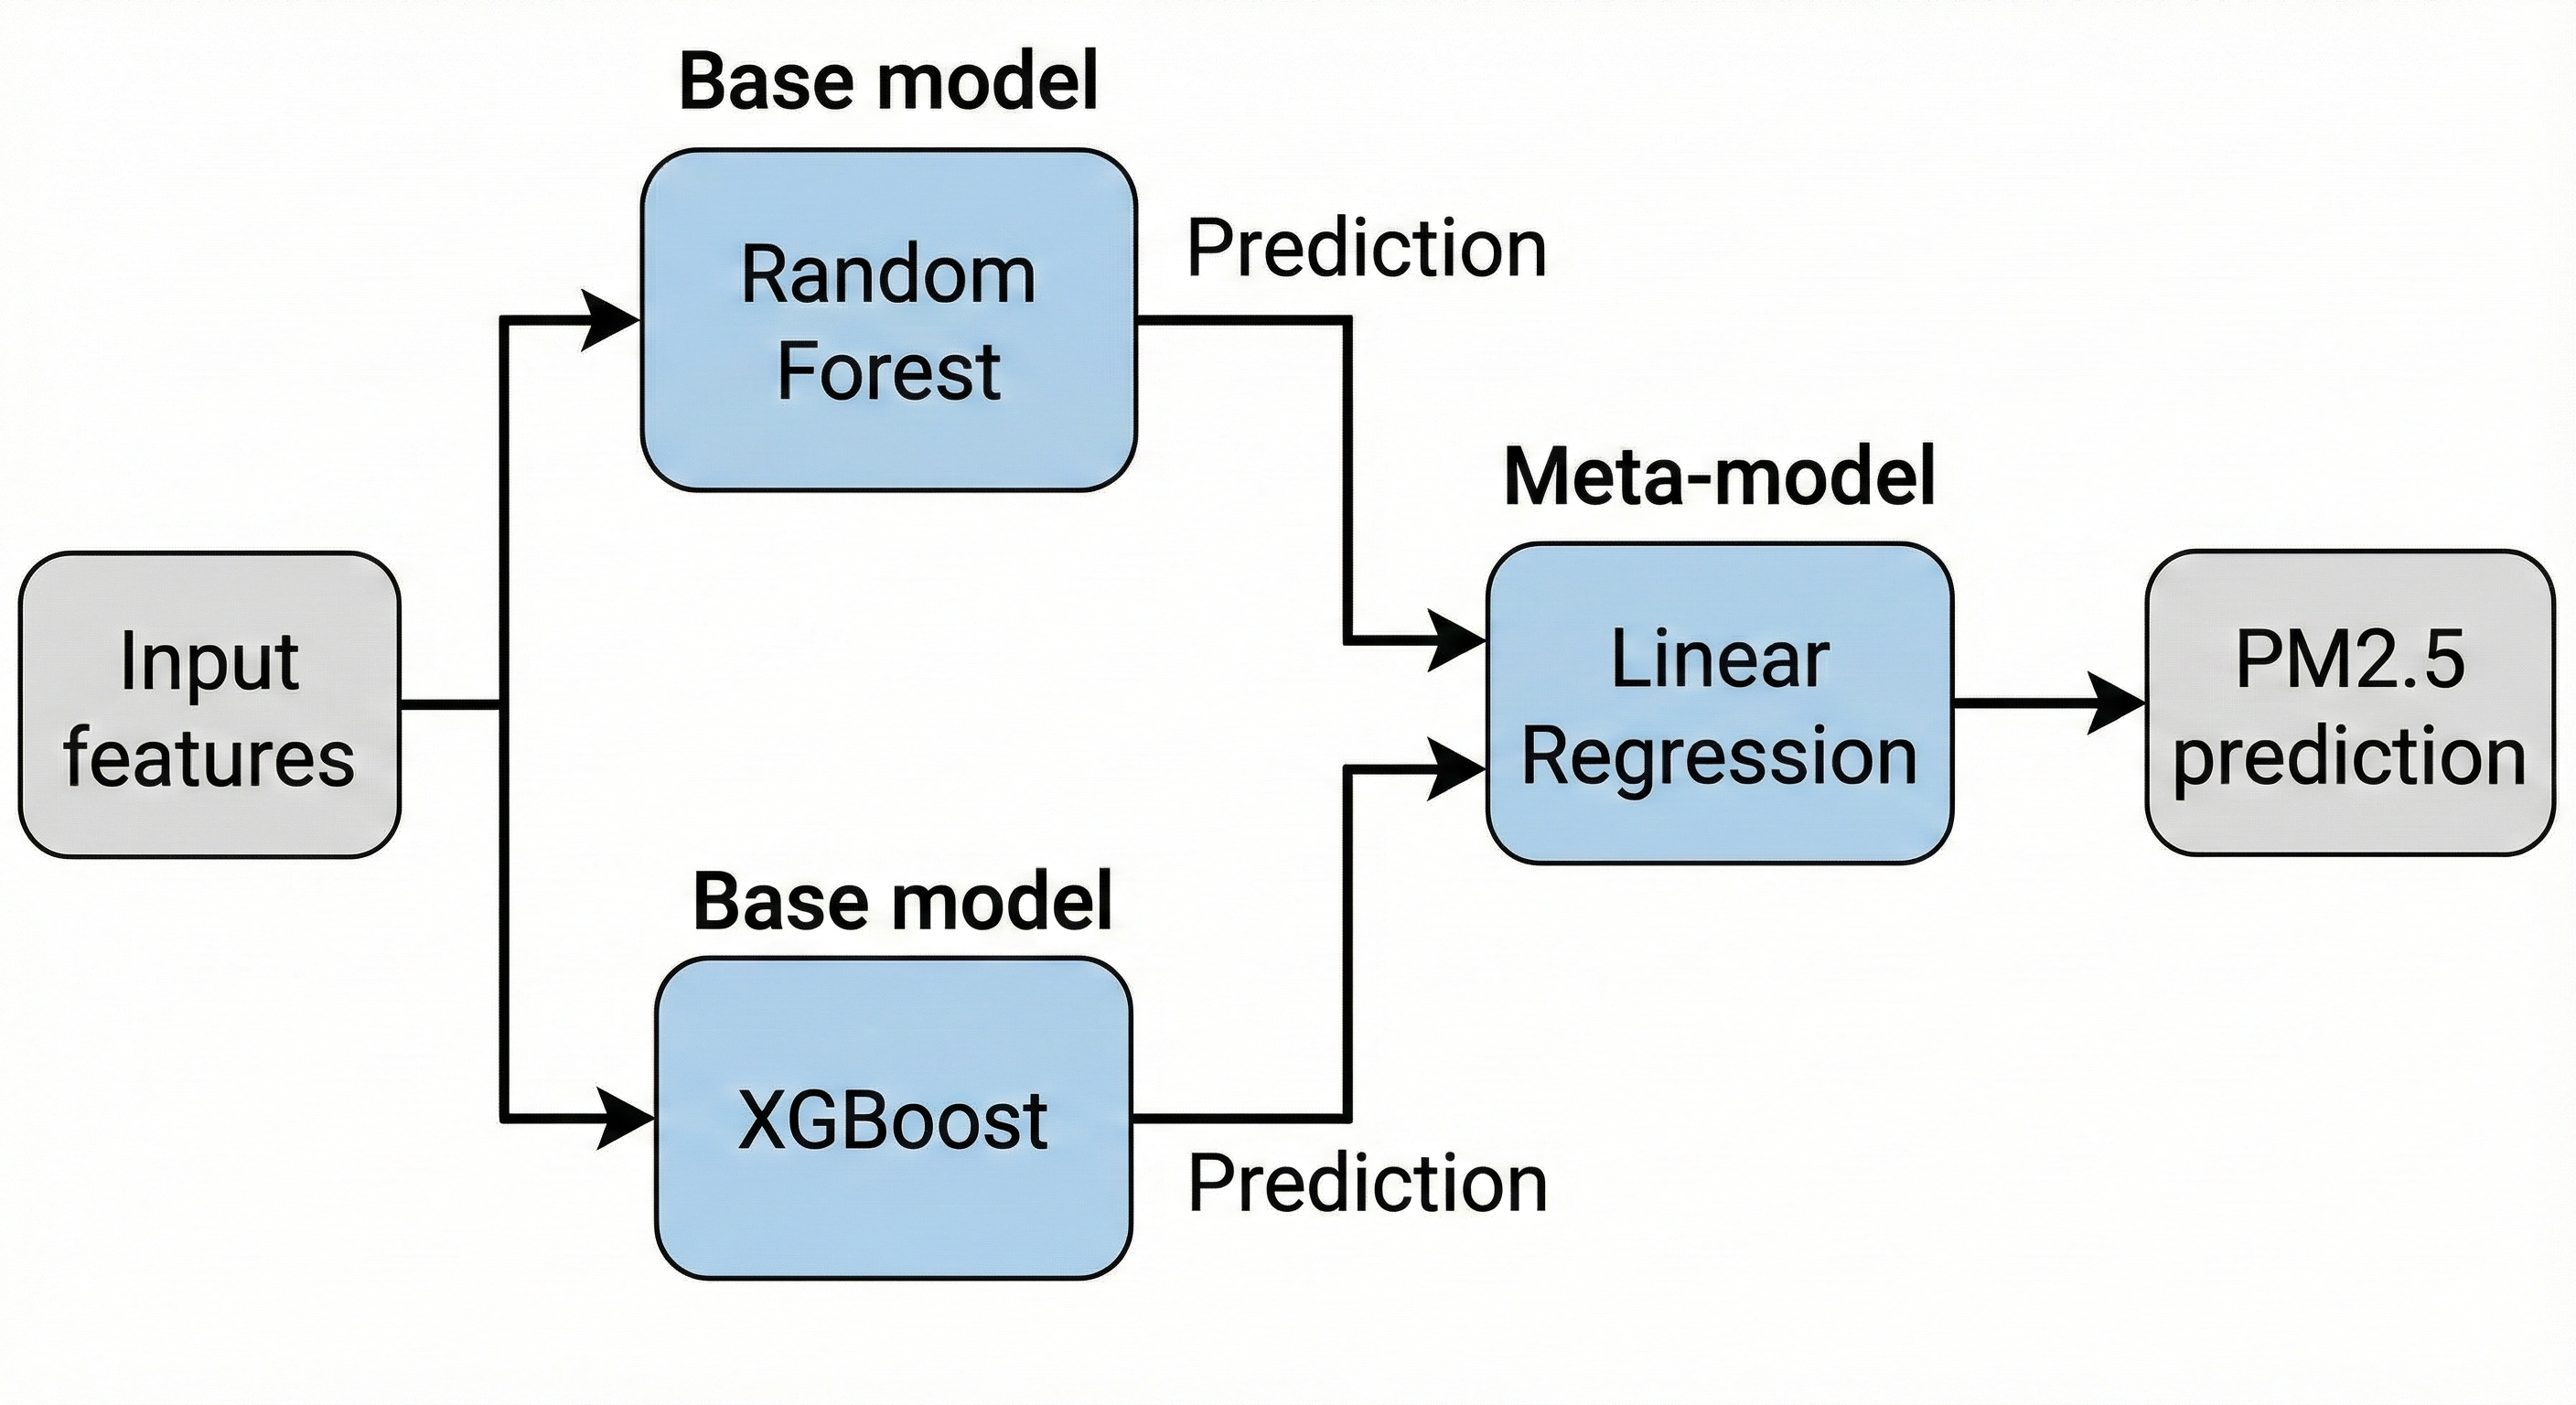
\includegraphics[width=\linewidth]{Gemini_Generated_Image_rwtb7vrwtb7vrwtb.png}
 % The suggested architecture for the Stacked Generalization Ensemble.  A Linear Regression meta-model takes the predictions from different base models (Random Forest and XGBoost) and uses them to make the final optimized PM2.5 forecast.
 % \label{fig:stacking_architecture}
 % \end{figure}



 % Data Sources and Collection
 % The model development employed a fused dataset that integrated ground-truth air quality observations with related satellite and meteorological variables.

 % Ground-Truth Data
 % The variable we want to predict is the PM2.5 concentration ($\mu g/m^3$).  This information came from a real-time air quality index dataset (CSV) that was used to train the algorithm.

 % Feature Data (Predictor Variables)
 % The predictor variables were obtained from a merged dataset that integrates ground measurements with data received from the Google Earth Engine (GEE) platform.  The last feature set ($X$) has six important variables:
 % \begin{itemize}
 % Satellite Data: Aerosol Optical Depth (AOD).
 % 1. Weather data: temperature (°C), the u-component of wind at 10m, and the v-component of wind at 10m.
 % Geospatial Data: Latitude and Longitude.
 % \end{itemize}

 % Data Preprocessing
 % To make sure the model was good, data preparation was done in the following steps:
 % 1.
 % 1. Missing Value Handling: Rows with missing ground-truth pollutant averages were taken out.  Also, any rows in the fused dataset that didn't have important predictor data, such AOD or Temperature, were removed.
 % Feature Standardization: We took raw geographic coordinate data (JSON strings) and turned it into separate floating-point columns for latitude and longitude.
 % Cleaning: Rows where coordinate extraction failed were taken out to make sure the dataset was the same.
 % \end{enumerate}



 % \begin{figure}[H] % [H] keeps it exactly here
 % \centering
 % 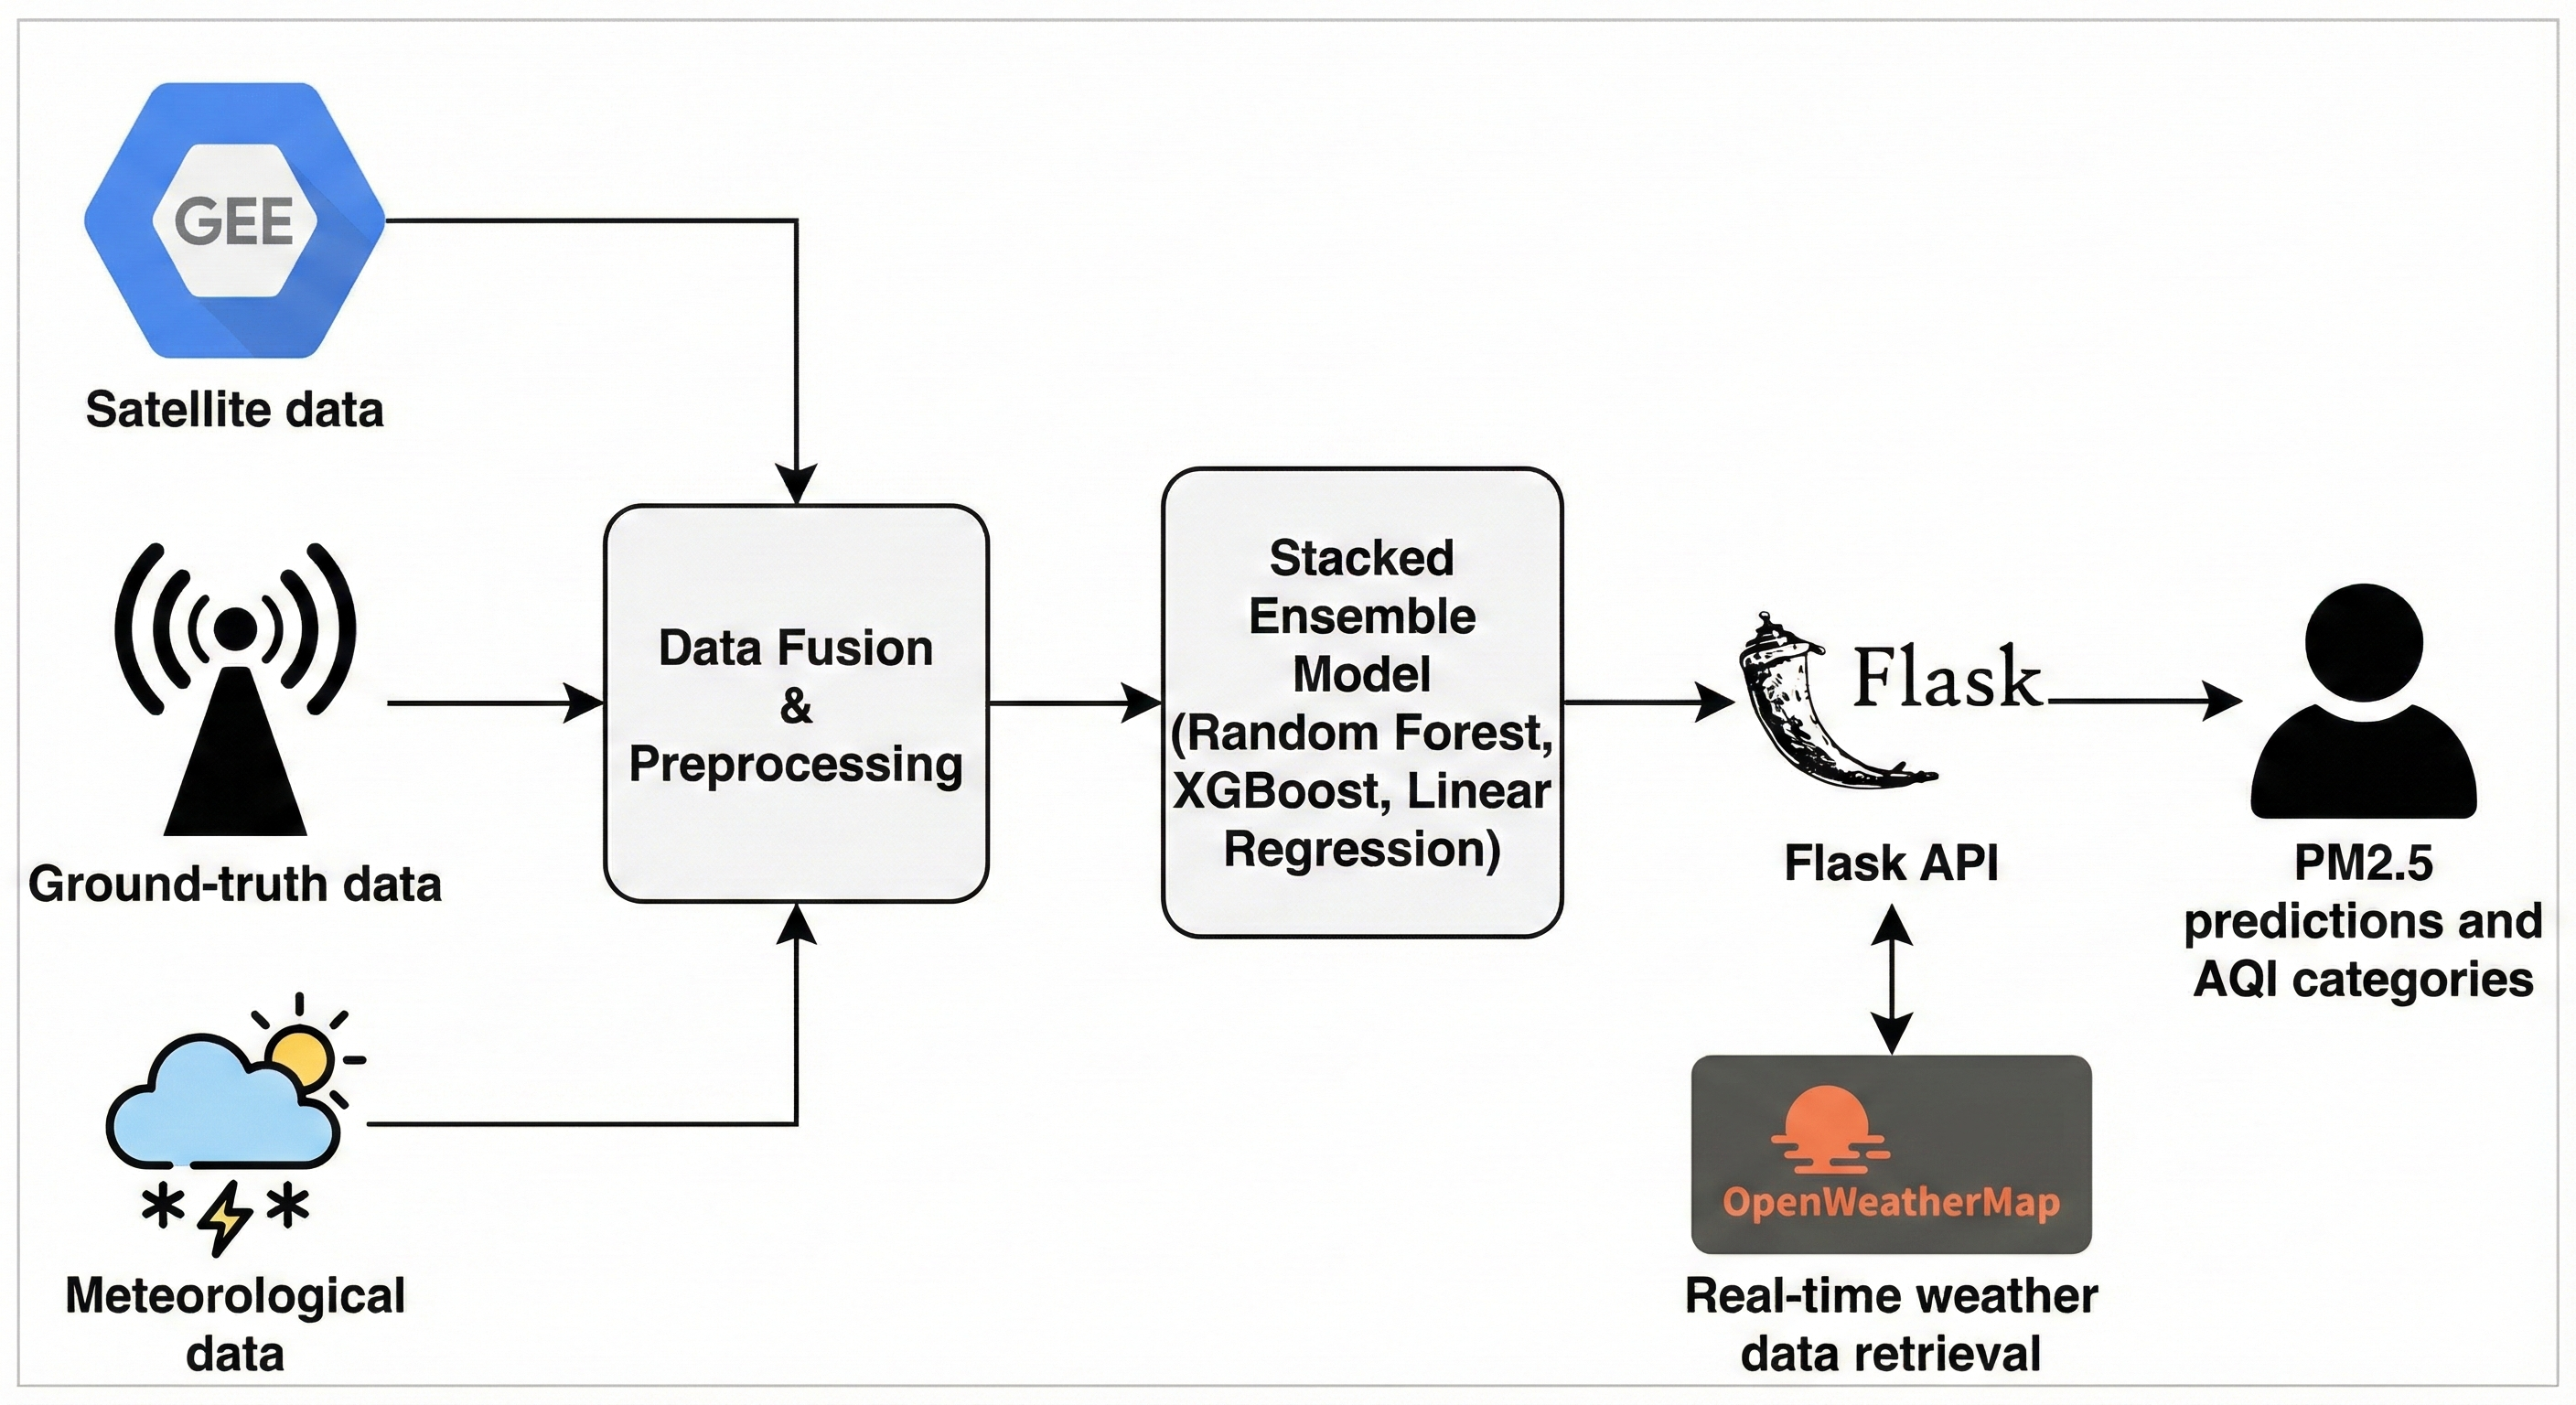
\includegraphics[width=\linewidth]{Gemini_Generated_Image_fvuvsifvuvsifvuv.png}
 % This is a whole data processing pipeline that shows how different types of data (satellite images, ground sensors, and meteorology) are brought in, cleaned, features are extracted, and all of this data is combined into one dataset for model training.
 % \label{fig:data_pipeline
 % \end{figure}



 % Subsection: Training and Testing the Model

 % Training Protocol
 % Using a random seed (`random_state=42`) to make sure the results could be repeated, the cleaned dataset was split into a training set (80%) and a testing set (20%).

 % There were two parts to the training process:
 % 1.
 % 1. Base Models: The Random Forest Regressor and XGBoost Regressor were both trained on the whole training feature set ($\mathbf{X}_{train}$) using `n_estimators=100`.
 % Meta-Model: Both basic models were used to make predictions for the test set.  We utilized these predictions ($\text{RF}_{pred}$ and $\text{XGB}_{pred}$) as features to train the Linear Regression meta-model against the real target values ($\mathbf{y}_{test}$).
 % \end{enumerate}

 % \subsection{Comparative Results (Test Set)}
 % We used R-squared (R2) and Root Mean Squared Error (RMSE) to see how well the model worked on the held-out test set.  The $R^2$ metric shows how much of the variance in the dependent variable can be predicted by the independent variables, whereas RMSE shows how big the error is on average.

 % Table \ref{tab:results} shows how well each base model did compared to the final stacked ensemble.

 % % FIX FOR TABLE PLACEMENT
 % \begin{table}[htbp]
 % \caption{Comparative Performance Metrics on the Test Set}
 % \label{tab:results}
 % In the middle
 % % ADD THIS LINE START %
 % \resizebox{\linewidth}{! }  
 % \begin{tabular}{lccc}
 % \toprule
 % Model R-squared ($R^2$) RMSE ($\mu g/m^3$) Role
 % \midrule
 % Random Forest Regressor & 0.5367 & 65.54 & Base Model \
 % XGBoost Regressor: 0.4276; 72.85; Base Model
 % Stacked Ensemble Model: 0.5592; --; Final Model:
 % The bottom rule
 % \end{tabular}
 % } % ADD THIS BRACKET END %
 % \end{table}

 % The Stacked Ensemble Model had the best $R^2$ score of $0.5592$, beating the base models Random Forest ($0.5367$) and XGBoost ($0.4276$).  This shows that stacking the strengths of several algorithms together makes predictions about PM2.5 concentrations more accurate.

 % \section{Structure for Deploying the System}
 % The system is set up as an API endpoint that can make real-time inferences in order to put the proposed methodology into action.  The logic for deployment goes like this:

 % 1.
 % 1. Input Collection: The system takes geographical coordinates (latitude and longitude) and the current Aerosol Optical Depth (AOD) from the user.
 % A real-time weather fetcher gets the needed meteorological parameters (Temperature, U-wind, V-wind) from the OpenWeatherMap API.
 % Feature Integration: Static inputs and dynamic weather data are combined into one feature vector that fits the training schema.
 % The Random Forest and XGBoost models use the feature vector to make predictions.  The Linear Regression meta-model uses their results to figure out the final PM2.5 concentration.
 % Classification: The projected concentration is put into the official Indian AQI categories (such Good, Moderate, Poor) and sent back as a JSON response.
 % \end{enumerate}


 % \begin{figure}[H] % [H] makes it stay right here
 % \centering
 % 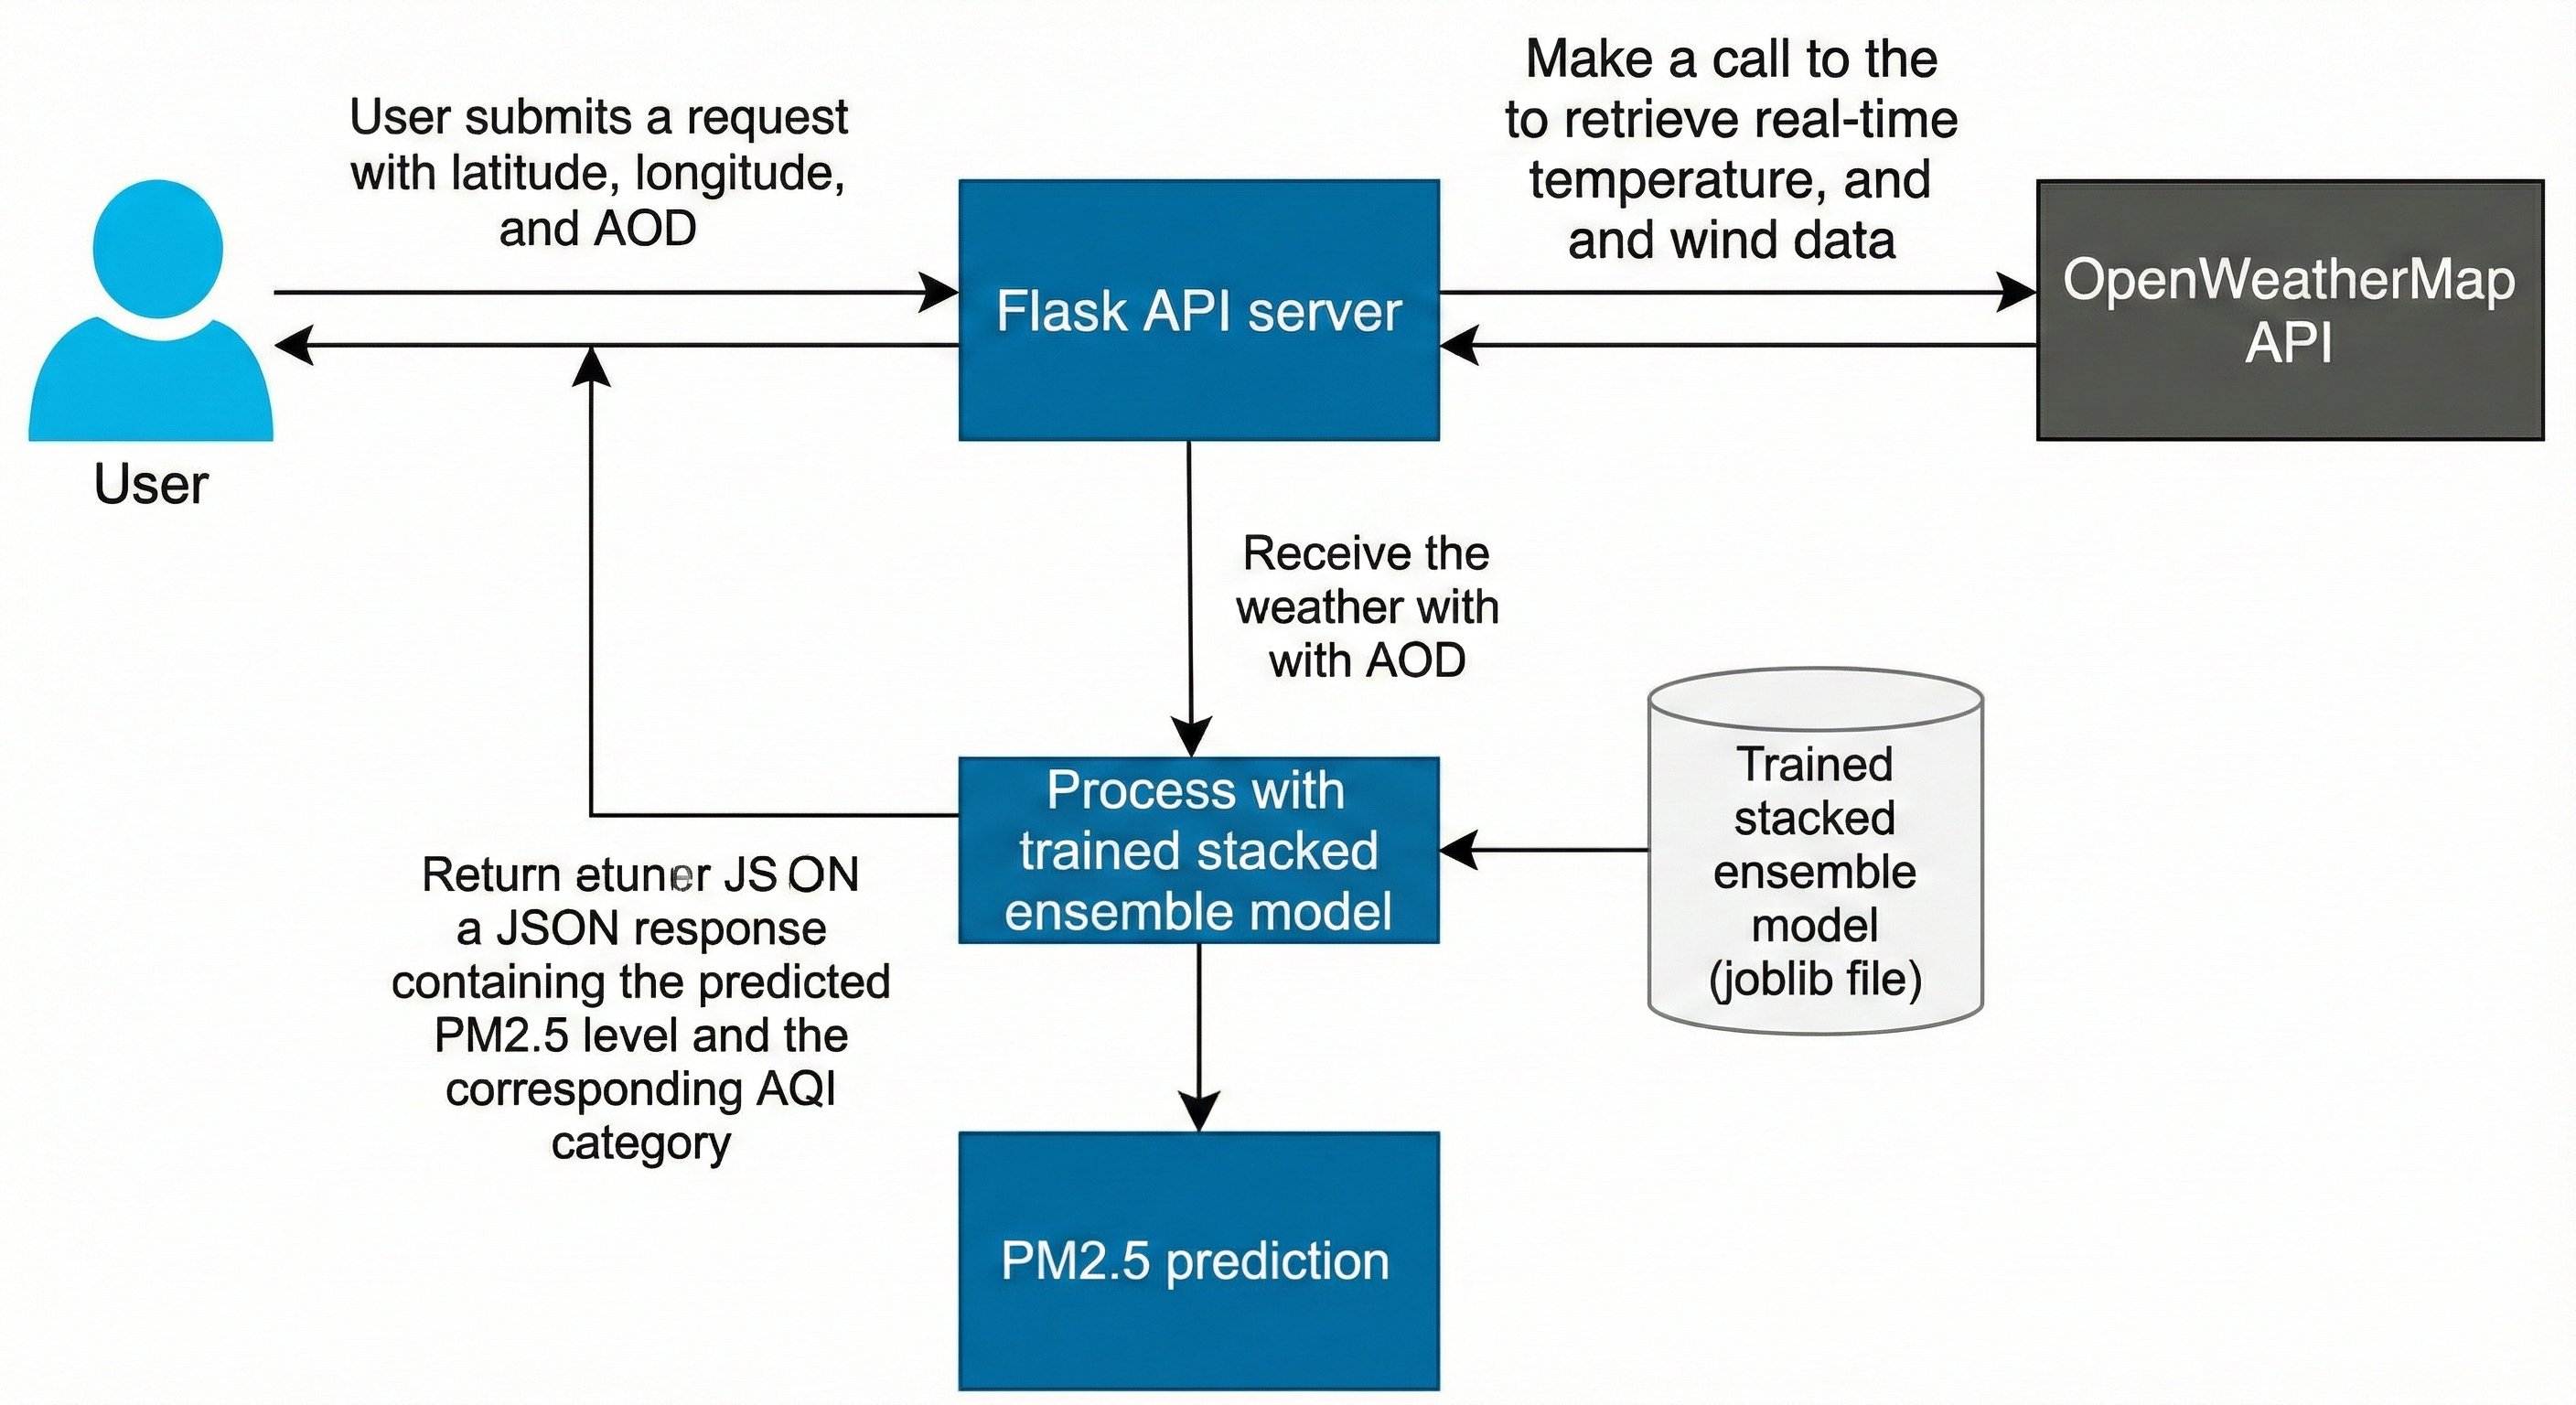
\includegraphics[width=\linewidth]{Gemini_Generated_Image_r6lm2ir6lm2ir6lm.png}
 % Caption: Structure for deploying an operational system.  As an API, the system accepts user location and AOD data, gets real-time weather, executes the layered prediction inference, and sends back a JSON response with the PM2.5 value and AQI category.
 % \label{fig:deployment_structure
 % \end{figure}



 % Results and Analysis

 % \subsection{Evaluation of Performance}
 % We used the Coefficient of Determination ($R^2$) and Root Mean Squared Error (RMSE) to assess the predictive models on a held-out test set ($20\%$).  The comparison results in Table \ref{tab:results} show that the ensemble method works well.

 % \begin{table}[htbp]
 % \centering
 % \caption{Comparison of Model Performance (Test Set)}
 % \label{tab:results}
 % \resizebox{\columnwidth}{! {
 % \begin{tabular}{lccc}
 % \toprule
 % Model & R2 Score & RMSE (μg/m3) & Improvement
 % |
 % XGBoost (Base) & 0.4276 & 72.85 & --
 % Random Forest (Base) & 0.5367 & 65.54 & +25.5% compared to XGB
 % Stacked Ensemble (SGE) & 0.5592 & -- & +4.2% versus RF
 % \bottomrule
 % \end{tabular}
 % }
 % \end{table}

 % The Stacked Generalization Ensemble (SGE) had the best prediction accuracy ($R^2=0.5592$), which was about 4.2% better than the best individual base model (Random Forest).  This shows that the linear meta-learner was able to use the strengths of the underlying models to their fullest, balancing the high variance of decision trees with the boosting power of XGBoost to lower the total generalization error.

 % Subsection: Importance and Drivers of Features
 % A look at the underlying decision trees shows a clear order of the things that affect $\text{PM}_{2.5}$ concentrations:

 % 1. 1. 1. 1. 1. 1. 1. 1.
 % 1. Aerosol Optical Depth (AOD): The most important part.  This confirms the physical link between satellite-observed atmospheric depth and ground-level particulate matter, showing that AOD is an important proxy for areas with few sensors.
 % Geospatial Variance: Latitude and Longitude came in second. They showed static regional emission sources (such industrial zones) and persistent dispersion patterns that dynamic weather data didn't show.
 % Wind components ($u, v$) and temperature made small modifications to the data, taking into consideration how pollutants move and build up over the course of a day.
 % \end{enumerate}

 % \subsection{Operational Usefulness}
 % The algorithm was able to convert continuous predictions to discrete **Indian AQI categories** (for example, "Satisfactory," "Moderate," or "Poor") in addition to its accuracy in regression.  This classification feature, which is available through the API, lets end users get health advice right away based on real-time data.


 % \section{Conclusion And Future Work}
 % \subsection{Conclusion

 % This study presented an ensemble-based machine learning framework for hyper-local PM$_{2.5}$ prediction by integrating various data sources, including ground-level observations, satellite-derived Aerosol Optical Depth (AOD), meteorological variables, and geographic information.  The suggested method uses a linear regression-based meta-model to merge Random Forest and XGBoost regressors. This takes use of their different learning styles to make predictions more accurate in areas where monitoring infrastructure is limited.

 % Testing on a separate test dataset showed that the ensemble framework works better than the individual basic models, with a $R^2$ value of about $0.56$.  These findings demonstrate that ensemble learning can improve PM$_{2.5}$ estimates when diverse data sources are successfully amalgamated, even if the overall performance improvements are minimal.  The analysis of feature importance showed that satellite-derived AOD and geographic location have the biggest effect on anticipated PM$_{2.5}$ concentrations. This shows how important it is to include remote sensing data and spatial context in air quality modeling.

 % The proposed system was shown to be useful in practice by being used as a real-time Flask-based application programming interface (API) in addition to being able to make predictions.  The system uses live weather data to make real-time PM$_{2.5}$ predictions and related Air Quality Index (AQI) categories. This shows that it might be used for operational air quality monitoring and decision assistance.

 % This research demonstrates that lightweight ensemble learning, when integrated with heterogeneous data fusion, provides a viable, interpretable, and computationally efficient approach for hyper-local PM$_{2.5}$ prediction.  Future study may concentrate on integrating temporal dynamics, supplementary pollutant variables, and more sophisticated spatiotemporal modeling methodologies to improve prediction precision and broaden forecasting potential.

 % Future Work
 % Following the success of this heterogeneous data fusion and ensemble-stacking method, further study may focus on other domains that enhance the model's precision, intricacy, and temporal applicability:

 % 1.
 % Integration of Spatiotemporal Modeling: The existing model relies on location as a fixed attribute.  Future study will concentrate on integrating cutting-edge deep learning architectures, including Graph Neural Networks (GNNs) and Convolutional Long Short-Term Memory (ConvLSTM) networks, to explicitly model intricate spatiotemporal connections and pollution transfer among various monitoring stations.
 % Advanced Feature Engineering: We will add new pollutants, such NO2 and SO2 (if we have them), to look at how pollutants interact with each other.  Also, adding time-based features (such month and hour of the day) to traffic and land-use data can greatly improve the feature space.
 % Hyperparameter Optimization and Model Tuning: The current SGE is performing well, but we will put in a lot of work to systematically optimize hyperparameters (for example, using Bayesian Optimization) for base models and meta-models in order to push the predictive limit of the stacked ensemble.
 % 1. Extending the Forecasting Horizon: Right now, the focus is on making predictions in real time.  Future study will concentrate on broadening the predicting horizon to 24, 48, and 72 hours.  This changes the use of the program from real-time monitoring to proactive air quality warning systems.
 % \end{enumerate}


 % \begin{thebibliography}{00}
 % Méndez, M., et al. (2023).  "Machine learning algorithms to forecast air quality: a survey." Artificial Intelligence Review 56(9): 10031-10066.
 % Zhang, Z., et al. (2024).  "A systematic survey of air quality prediction based on deep learning." Alexandria Engineering Journal 93: 128-141.

 % Lee, J.-B., et al. (2022).  "Development of a deep neural network for predicting 6 h average PM 2.5 concentrations up to 2 subsequent days using various training data." Geoscientific Model Development 15(9): 3797-3813.

 % Pan, R., et al. (2024).  "A Graph Attention Recurrent Neural Network Model for PM2.5 Prediction: A Case Study in China from 2015 to 2022." Atmosphere 15(7): 799.
 % \bibitem{b5}Zhang, Z.  and S.  Zhang (2023).  "Modeling air quality PM2.5 forecasting using deep sparse attention-based transformer networks." International Journal of Environmental Science and Technology 20(12): 13535-13550.

 % Qi, Y., et al. (2019).  "A hybrid model for spatiotemporal forecasting of PM2.5 based on graph convolutional neural network and long short-term memory." Science of the Total Environment 664: 1-10.

 % Utku, A., et al. (2025).  "Advancing Air Quality Monitoring: Deep Learning-Based CNN-RNN Hybrid Model for PM2.5 Forecasting." Atmosphere 16(9): 1003.
 % Das, A.  (2021).  "A hybrid deep learning model for predicting air quality time series." Indonesian Journal of Electrical Engineering and Computer Science.
 % \end{thebibliography}
 % \vspace{12pt
 % \color{red}

 % \end{document}